% ***************************************************
% Appendix
% ***************************************************
\chapter{Supplementary figure for Chapter 5}

Quantifying phylogenetic signal requires an independently-derived
reference phylogeny as a yardstick. Our reference phylogeny is a 285-tip
Pama-Nyungan phylogeny inferred by the second author. Figure S1 gives a
112-tip subset of this phylogeny, corresponding to the 112 doculects
used in this study.

\begin{figure}
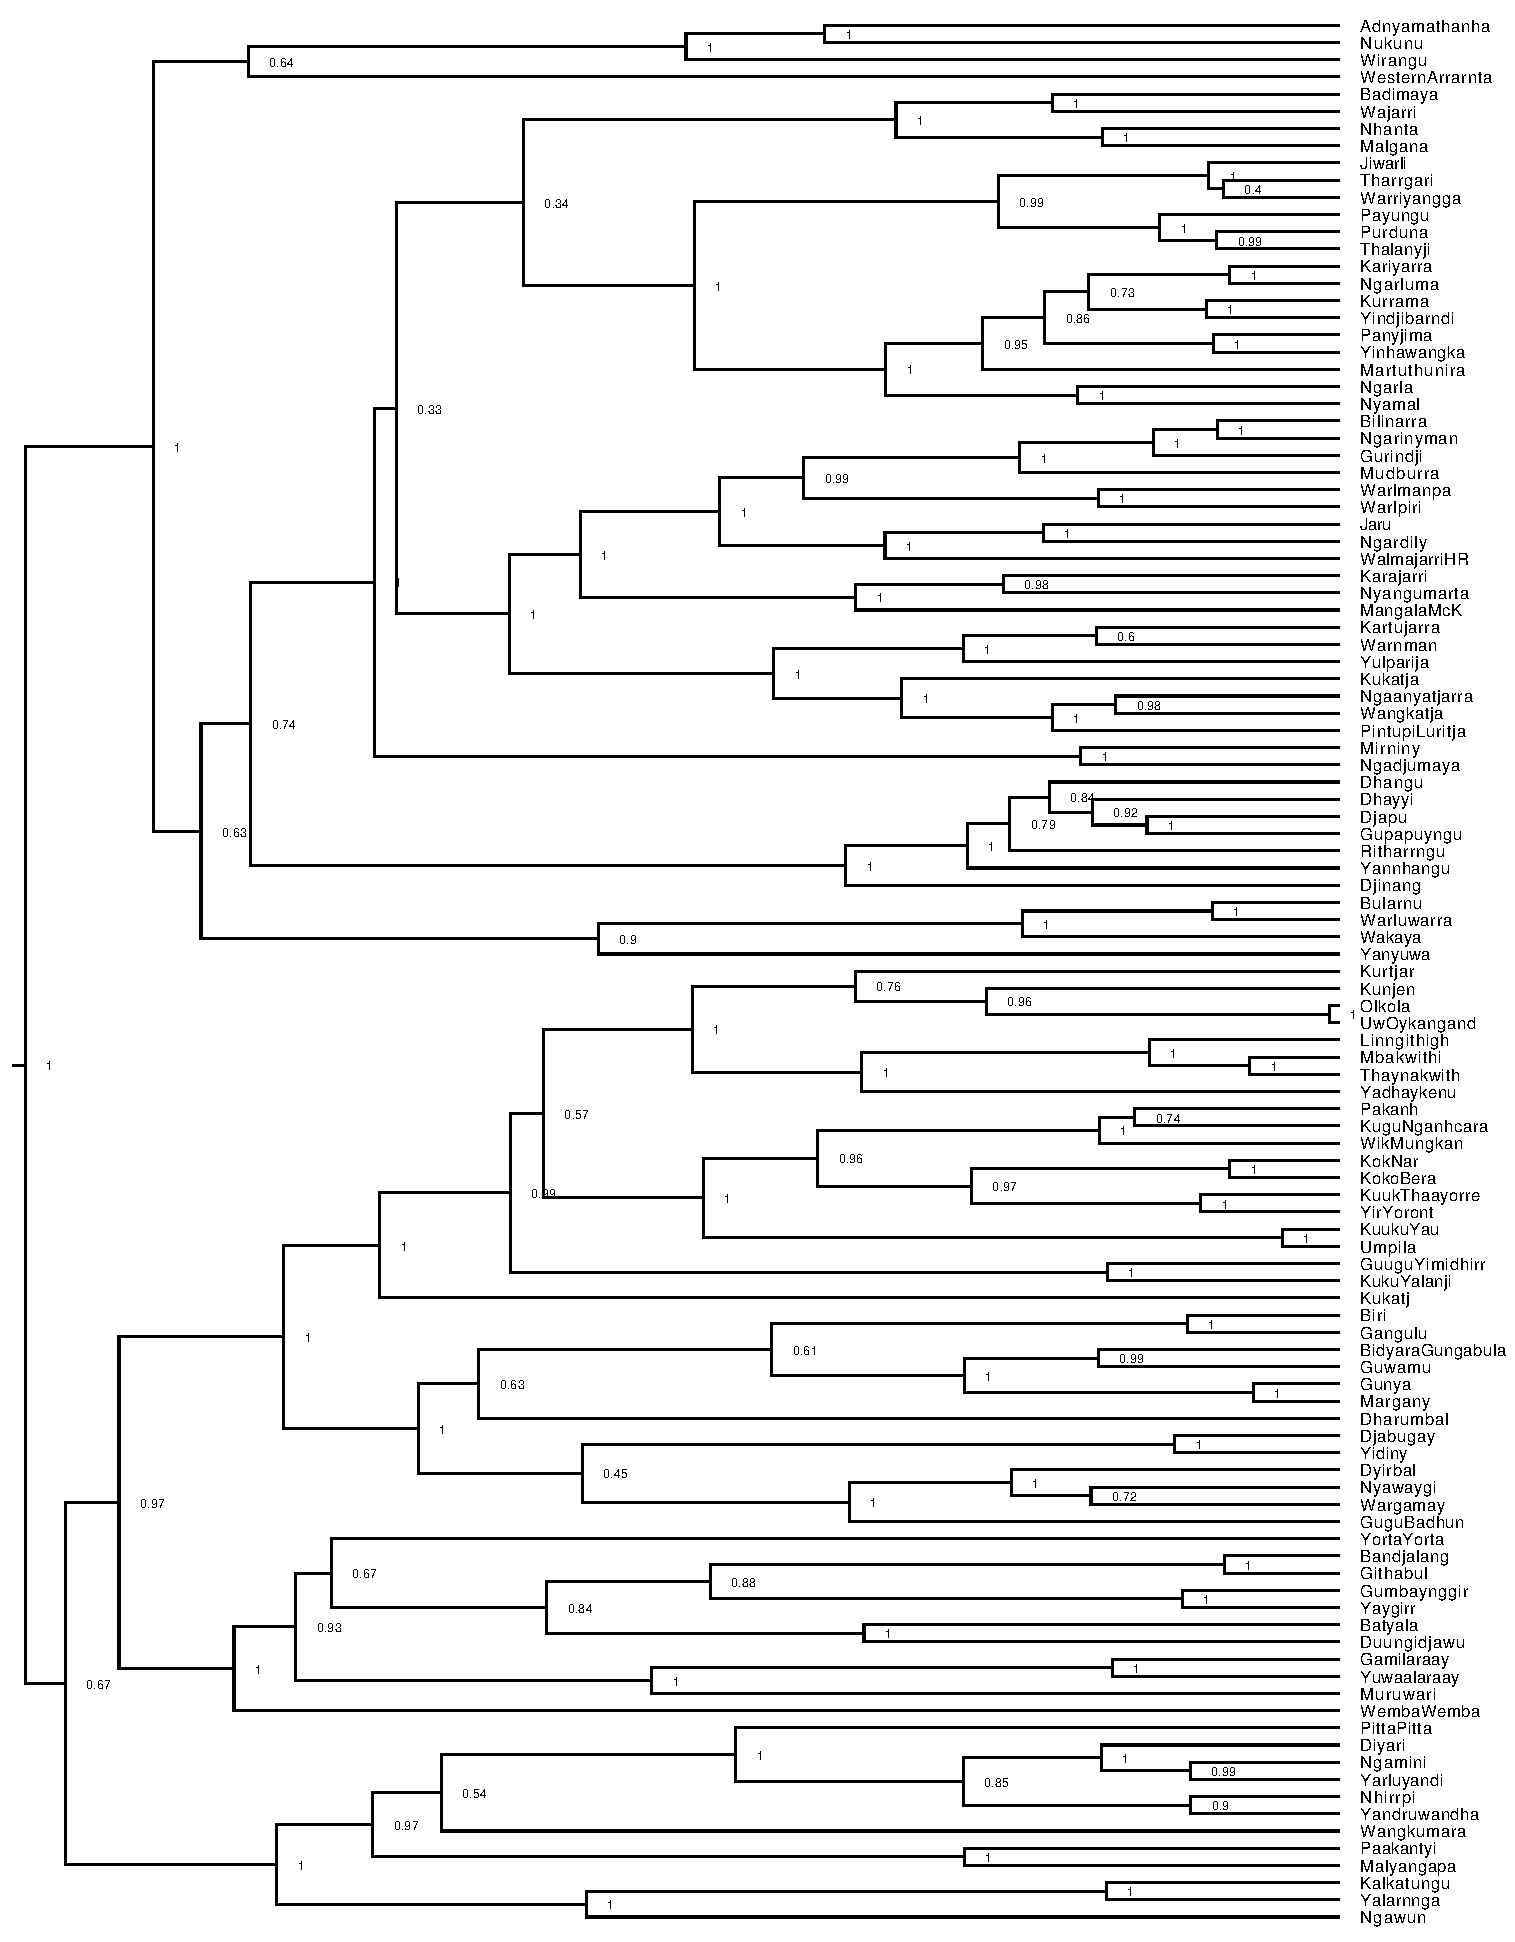
\includegraphics[width=1\linewidth]{Appendix-A/fig/PN_beast_pruned} \caption[Pama-Nyungan reference phylogeny]{Pama-Nyungan reference phylogeny. Node labels are posterior probabilities, giving an indication of support for each node. Although there is no strict, conventional cut-off, clades with posterior values above 0.5 are considered supported and values above 0.8 are considered strongly supported (Bowern \& Atkinson 2012, p. 829).}\label{fig:plot-ref-tree2}
\end{figure}

As discussed in the main paper, the reference phylogeny was constructed
using Bayesian phylogenetic methods in the software BEAST2
\autocite{bouckaert_beast_2014}. Bayesian phylogenetic methods use a
Markov Chain Monte Carlo (MCMC) procedure to efficiently search the
hypothesis space of possible trees and return a large posterior sample
of similarly credible alternatives (capturing phylogenetic uncertainty).
The tree in Figure S1 above is a maximum clade credibility tree, which
is a summation of the posterior sample where the likelihood of all nodes
in the tree (in terms of how frequently a given node reappears across
the posterior sample) is maximized.

For further details on the Pama-Nyungan phylogeny used as a reference
phylogeny in this study, see \textcite{bowern_pama-nyungan_2015}. See
also \textcite{bowern_computational_2012}, which infers a Pama-Nyungan
phylogeny in the same way, using exactly the same evolutionary model
parameters, but with an earlier iteration of the dataset containing
fewer doculects. Additional discussion of the general process of
constructing language phylogenies in BEAST2 can be found in
\textcite{bouckaert_origin_2018}, although a different evolutionary
model is used.

The reference phylogeny was inferred using lexical cognate data, coded
according to the principles of the Comparative Method. The cognate data
used in the reference phylogeny is publicly available on Zenodo
\autocite{bowern_pama-nyungan_2018} and also as a subset of the
305-language dataset in \textcite{bouckaert_origin_2018}. This latter
source also includes a Perl script for converting multistate cognate
judgements into a binary matrix for use with BEAST2 phylogenetic
software and will include information on underlying sources.
